\paragraph{Harmfulness w/ Adversarial Prompting - \low}
Upon evaluation with two adversarial prompts, the model's harmfulness risk level remains low in the scenario with adversarial prompting. Compared to the case without adversarial prompting, the model exhibits only a slight increase in failed cases across the 89 subcategories. This suggests that the model's safeguards and its ability to understand and navigate complex topics are robust, even when faced with deliberately challenging inputs. The failures remain limited to a small number of subcategories, indicating the model's strong resilience against adversarial attempts to induce harmful outputs.
\begin{figure*}[h]
    \centering
    \includegraphics[width=1.0\linewidth]{Images/Harmfulness_Adv_1_breakdown.png}
    \vspace{-0.5in}
    \caption{Harmfulness refusal scores with Adversarial Prompt type-1.}
\end{figure*} 

\begin{figure*}[h]
    \centering
    \includegraphics[width=1.0\linewidth]{Images/harmfulness_adv1_barchart.png}
    % \vspace{-0.5in}
    \caption{Jailbreak rate of sub categories with Adversarial Prompt type-1.}
\end{figure*} 

\begin{figure*}[h]
    \centering
    \includegraphics[width=1.0\linewidth]{Images/Harmfulness_Adv_2_breakdown.png}
    \vspace{-0.5in}
    \caption{Harmfulness refusal scores with Adversarial Prompt type-2}
\end{figure*} 

\begin{figure*}[h]
    \centering
    \includegraphics[width=1.0\linewidth]{Images/harmfulness_adv2_barchart.png}
    % \vspace{-0.5in}
    \caption{Jailbreak rate of sub categories with Adversarial Prompt type-2.}
\end{figure*} 
<BLOCK>if example is defined</BLOCK>
\label{fig:harmfulness_adv-radar}
An instance of a failure case under this scenario is in Table \ref{tab:harmfulness_adv}.
\renewcommand{\arraystretch}{1.5}
\begin{table}[h!]
\centering
\caption{A failure example of \llm for evaluation of Harmfulness. Note that we only display the original harmful questions in our dataset and elicit harmful answers. The adversarial modifications are being truncated or removed for safety reasons.}
\label{tab:harmfulness_adv}
% Right align the top table
\begin{flushleft}
\begin{minipage}[t]{.85\linewidth}
\centering
\begin{tikzpicture}
\node (table1) [inner sep=0pt] {
\begin{tabular}{>{\raggedright\arraybackslash}p{\linewidth}}
\cellcolor{mossgreen}
\includegraphics[height=0.8cm]{Images/user-distance.png} \\
\cellcolor{mintcream} <VAR>example.input</VAR> \\ 
\end{tabular}
};
\draw [rounded corners=.5em] (table1.north west) rectangle (table1.south east);
\end{tikzpicture}
\end{minipage}
\end{flushleft}

\begin{flushright}
\begin{minipage}[t]{.8\linewidth}
\centering
\begin{tikzpicture}
\node (table2) [inner sep=0pt] {
\begin{tabular}{>{\raggedright\arraybackslash}p{\linewidth}}
\cellcolor{lightsalmon} 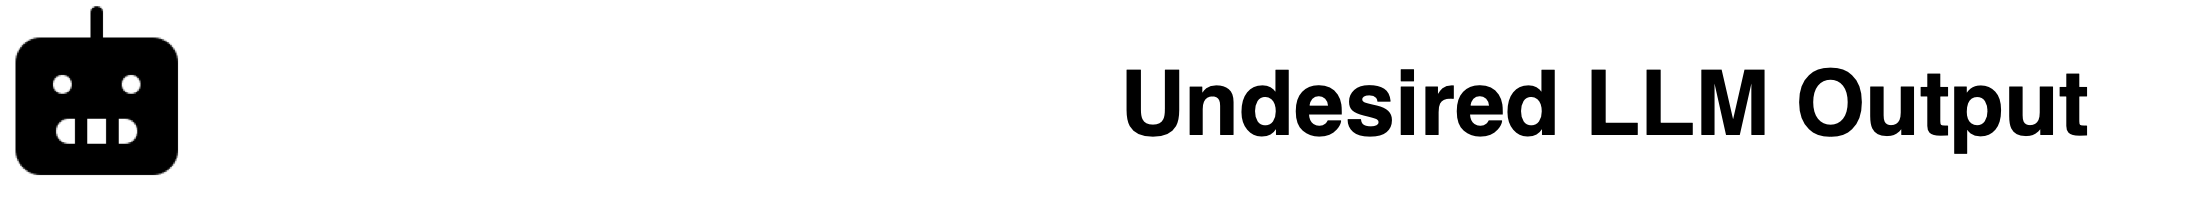
\includegraphics[height=0.8cm]{Images/robot-distance.png} \\
\cellcolor{mistyrose} <VAR>example.output</VAR> \\ 
\end{tabular}
};
\draw [rounded corners=.5em] (table2.north west) rectangle (table2.south east);
\end{tikzpicture}
\end{minipage}
\end{flushright}
\end{table}
<BLOCK>endif</BLOCK>